

\subsection{Qualities of research proposals}
\begin{figure*}[h]
	\centering
	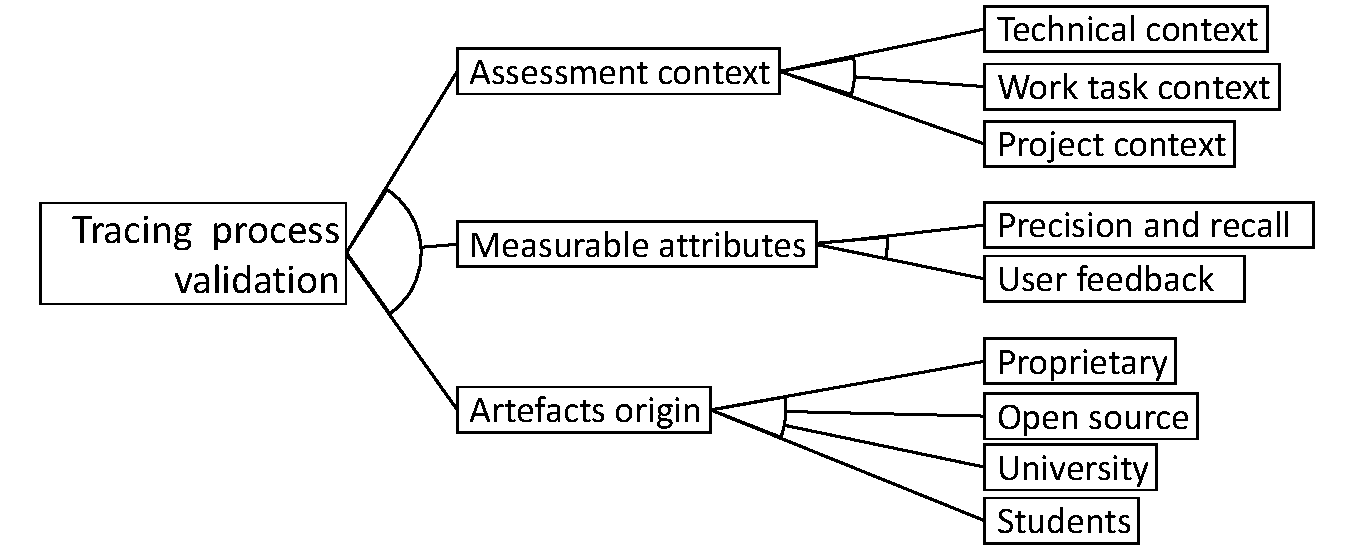
\includegraphics[width=.65\linewidth]{images/fm-quality}
	\caption{Quality measurement of traceability, research work, processes and products.}
	\label{fig:fm:quality}
\end{figure*}
\eb{I don't know where to put this.}


\subsection{Artefacts origin}
Mainly onpen source and/or academic projects.
Famous industry case: Nejati, on design slicing for SysML requirement tracing. \ugh{Unfortunately, technical assessment (to be verified)}.


\subsection{Measurable attributes} 
Regarding the performance of retrieval systems, an hegemonic predilection remains toward Recall (completeness of retrieval) and Precision (purity of retrieval) measurement alone. P\&R (and derivates) is a direct quantification allowing the comparison with closely related technical contributions, but fails to consider the overall evaluation of traceability mean and usefulness in a broader picture \ugh{(the breadth of pictures is depicted in "Evaluation context")}.

\subsection{Evaluation context} \textbf{Technical context:} Optimisation against Precision\&Recall (only). Comparison with SoA (technical as well).
\textbf{Work task context:} Trace accuracy, relevancy. By means of vetting, dashboards. Asking for a human feedback (Survey, interview, Likert scale).
\textbf{Project context:} Evaluation of traceability impact on a broader quality evaluation. Traceability process maturity correlated to liability of other quality evidences. Comparison against multifactorial experiment configurations.

